\documentclass[tikz,border=6pt]{standalone}
\usepackage{amsmath,amssymb}
\usetikzlibrary{arrows.meta,calc}
\definecolor{ink}{HTML}{102B42}
\definecolor{bluefill}{HTML}{DFEFFE}
\definecolor{greenfill}{HTML}{DEF6D6}
\definecolor{yellowfill}{HTML}{D1F7FF}
\definecolor{pinkfill}{HTML}{FCCCDA}
\begin{document}
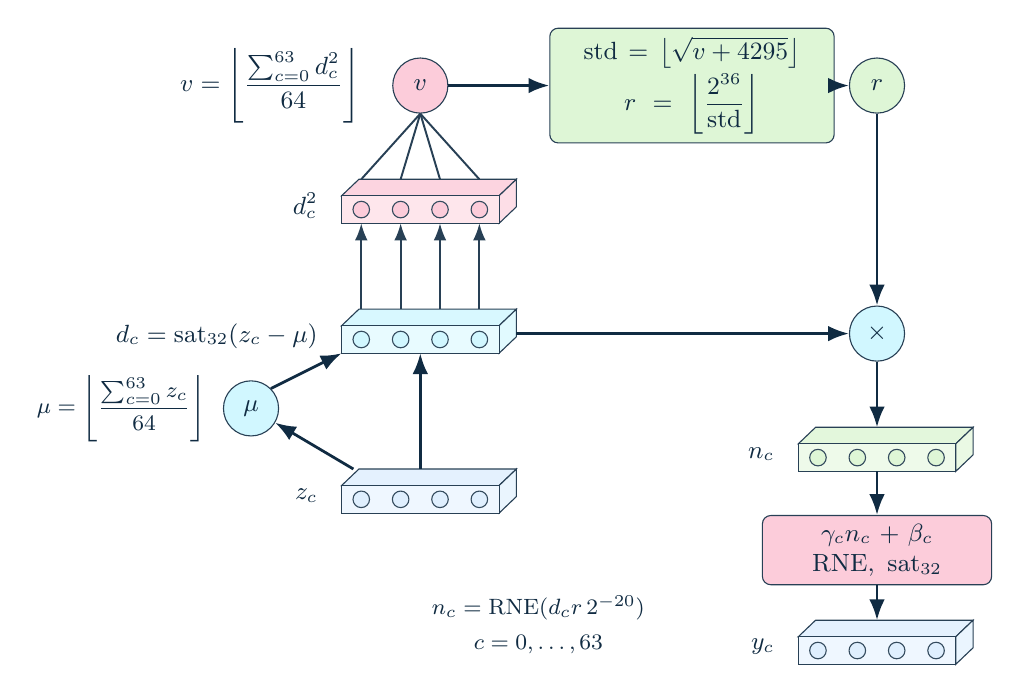
\begin{tikzpicture}[font=\small,text=ink,>=Latex,
 arr/.style={->,draw=ink,line width=1pt},
 link/.style={draw=ink!90,line width=.7pt},
 box/.style={draw=ink!90,rounded corners=3pt,align=center,inner sep=3pt,fill=greenfill},
 dot/.style={circle,draw=ink!90,fill=yellowfill,minimum size=7mm,inner sep=0pt}]
% A row vector is shown as a shallow three-dimensional block.
\newcommand{\vectorblock}[4]{%
 \begin{scope}[shift={(#1,#2)}]
 \filldraw[fill=#3!85,draw=ink!90] (0,.35)--(.22,.56)--(2.22,.56)--(2,.35)--cycle;
 \filldraw[fill=#3!65,draw=ink!90] (2,0)--(2.22,.21)--(2.22,.56)--(2,.35)--cycle;
 \filldraw[fill=#3!50,draw=ink!90] (0,0) rectangle (2,.35);
 \foreach \x in {.25,.75,1.25,1.75}{\filldraw[fill=#3,draw=ink!85] (\x,.175) circle (.105);}
 \node[anchor=east,align=right] at (-.18,.22) {#4};
 \end{scope}}
% Left column: vector transforms and reduction.
\vectorblock{0}{-.38}{bluefill}{$z_c$}
\vectorblock{0}{1.65}{yellowfill}{$d_c=\operatorname{sat}_{32}(z_c-\mu)$}
\vectorblock{0}{3.3}{pinkfill}{$d_c^2$}
\node[dot,fill=yellowfill] (mean) at (-1.15,.95) {$\mu$};
\draw[arr] (1,.18)--(1,1.65);
\draw[arr] (.15,.18)--(mean);
\draw[arr] (mean.north east)--(0,1.65);
\node[anchor=east,font=\footnotesize,align=right] at (-1.6,.95) {$\displaystyle\mu=\left\lfloor\frac{\sum_{c=0}^{63}z_c}{64}\right\rfloor$};
\foreach \x in {.25,.75,1.25,1.75}{\draw[link,->] (\x,2.21)--(\x,3.3);}

\node[dot,fill=pinkfill] (var) at (1,5.05) {$v$};
\foreach \x in {.25,.75,1.25,1.75}{\draw[link] (\x,3.86)--(var.south);}
\node[anchor=east,align=right] at (.35,5.05) {$\displaystyle v=\left\lfloor\frac{\sum_{c=0}^{63}d_c^2}{64}\right\rfloor$};
% Top: a scalar computation shared by all channels.
\node[box,text width=34mm] (inverse) at (4.45,5.05) {$\displaystyle\mathrm{std}=\left\lfloor\sqrt{v+4295}\right\rfloor$\\[1pt]$\displaystyle r=\left\lfloor\frac{2^{36}}{\mathrm{std}}\right\rfloor$};
\draw[arr] (var)--(inverse);
% Right column: shared scalar times the centered vector, then affine output.
\node[dot,fill=greenfill] (factor) at (6.8,5.05) {$r$};
\draw[arr] (inverse)--(factor);
\node[dot] (mul) at (6.8,1.9) {$\times$};
\draw[arr] (factor)--(mul);
\draw[arr] (2.22,1.9)--(mul);
\vectorblock{5.8}{.15}{greenfill}{$n_c$}
\draw[arr] (mul)--(6.8,.71);
\node[box,fill=pinkfill,text width=27mm] (affine) at (6.8,-.85) {$\gamma_c n_c+\beta_c$\\$\operatorname{RNE},\ \operatorname{sat}_{32}$};
\draw[arr] (6.8,.15)--(affine);
\vectorblock{5.8}{-2.3}{bluefill}{$y_c$}
\draw[arr] (affine)--(6.8,-1.74);
\node[align=center,font=\footnotesize] at (2.5,-1.8) {$n_c=\operatorname{RNE}(d_c r\,2^{-20})$\\[3pt]$c=0,\ldots,63$};
\end{tikzpicture}
\end{document}
